% !TEX TS-program = pdflatex
% !TEX encoding = UTF-8 Unicode

% This file is a template using the "beamer" package to create slides for a talk or presentation
% - Talk at a conference/colloquium.
% - Talk length is about 20min.
% - Style is ornate.

% MODIFIED by Jonathan Kew, 2008-07-06
% The header comments and encoding in this file were modified for inclusion with TeXworks.
% The content is otherwise unchanged from the original distributed with the beamer package.

\documentclass{beamer}


% Copyright 2004 by Till Tantau <tantau@users.sourceforge.net>.
%
% In principle, this file can be redistributed and/or modified under
% the terms of the GNU Public License, version 2.
%
% However, this file is supposed to be a template to be modified
% for your own needs. For this reason, if you use this file as a
% template and not specifically distribute it as part of a another
% package/program, I grant the extra permission to freely copy and
% modify this file as you see fit and even to delete this copyright
% notice. 


\mode<presentation>{
	\usetheme{Warsaw}
		% or ...
	\setbeamercovered{transparent}
		% or whatever (possibly just delete it)
}

%\usepackage[spanish]{babel}
\usepackage[english]{babel}
%\selectlanguage{spanish}
\usepackage{bold-extra}
% or whatever

\usepackage[utf8]{inputenc}
% or whatever

\usepackage{times}
\usepackage[T1]{fontenc}
% Or whatever. Note that the encoding and the font should match. If T1
% does not look nice, try deleting the line with the fontenc.

\usepackage{graphicx}
\graphicspath{{./images/}{./presentation-files/images/}}
\usepackage{tikz}

\usepackage{multicol}

\title[AutoSA]{AutoSA: sistema para automatizar las órdenes de reposición en el Sistema de Abastecimiento del Instituto de Salud Pública de México}

%\subtitle
%{Include Only If Paper Has a Subtitle}

\author{Ernesto Carrillo Espinosa}
% - Give the names in the same order as the appear in the paper.
% - Use the \inst{?} command only if the authors have different
%   affiliation.

\institute{
  Facultad de Ciencias\\
  Universidad Nacional Autónoma de México
}
% - Use the \inst command only if there are several affiliations.
% - Keep it simple, no one is interested in your street address.

\date{15 de enero de 2020}
% - Either use conference name or its abbreviation.
% - Not really informative to the audience, more for people (including
%   yourself) who are reading the slides online

\subject{Presentación del sistema AutoSA}
% This is only inserted into the PDF information catalog. Can be left
% out. 



% If you have a file called "university-logo-filename.xxx", where xxx
% is a graphic format that can be processed by latex or pdflatex,
% resp., then you can add a logo as follows:

%\pgfdeclareimage[height=0.5cm]{university-logo}{unam-blanco}
%\logo{\pgfuseimage{university-logo}}
%\logo{\includegraphics[scale=0.1]{unam-negro}}


% Delete this, if you do not want the table of contents to pop up at
% the beginning of each subsection:
\AtBeginSection[]{
%\AtBeginSubsection[]{
	\begin{frame}<beamer>{Índice}
		\begin{multicols}{2}
		\tableofcontents[currentsection,currentsubsection]
		\end{multicols}
	\end{frame}
}

% If you wish to uncover everything in a step-wise fashion, uncomment
% the following command: 

%\beamerdefaultoverlayspecification{<+->}

% Version de PDF
%\pdfminorversion=7

\begin{document}
\addtobeamertemplate{headline}{}{
	\begin{tikzpicture}[remember picture,overlay]
		\node[anchor=north west,yshift=0pt] at (current page.north west){
			
\includegraphics[height=1.3cm]{unam-blanco}
		};
		\node[anchor=north east,yshift=0pt] at (current page.north east){
			
\includegraphics[height=1.3cm]{ciencias-blanco}
		};
	\end{tikzpicture}
}

% Slide de título
\begin{frame}
	\titlepage
\end{frame}

% Índice
\begin{frame}{Índice}
	\begin{multicols}{2}
	\tableofcontents
	\end{multicols}
  % You might wish to add the option [pausesections]
\end{frame}

\section{Introducción}
\subsection{Contexto}
	\begin{frame}{Actores}
		\begin{block}{Instituto de Salud}
			Realiza la solicitud de medicamentos mediante \textit{órdenes de reposición}.
		\end{block}
		\begin{block}{Sistema de Abastecimiento}
			Sistema web por el cual el Instituto de Salud realiza las órdenes de reposición.
		\end{block}
		\begin{block}{Farmacéutica}
			Quien provee medicamentos al Instituto de Salud.
		\end{block}
	\end{frame}

\subsubsection{Procesos}
	\begin{frame}{Envío de órdenes de reposición}
		\begin{figure}[H]
		\centering
		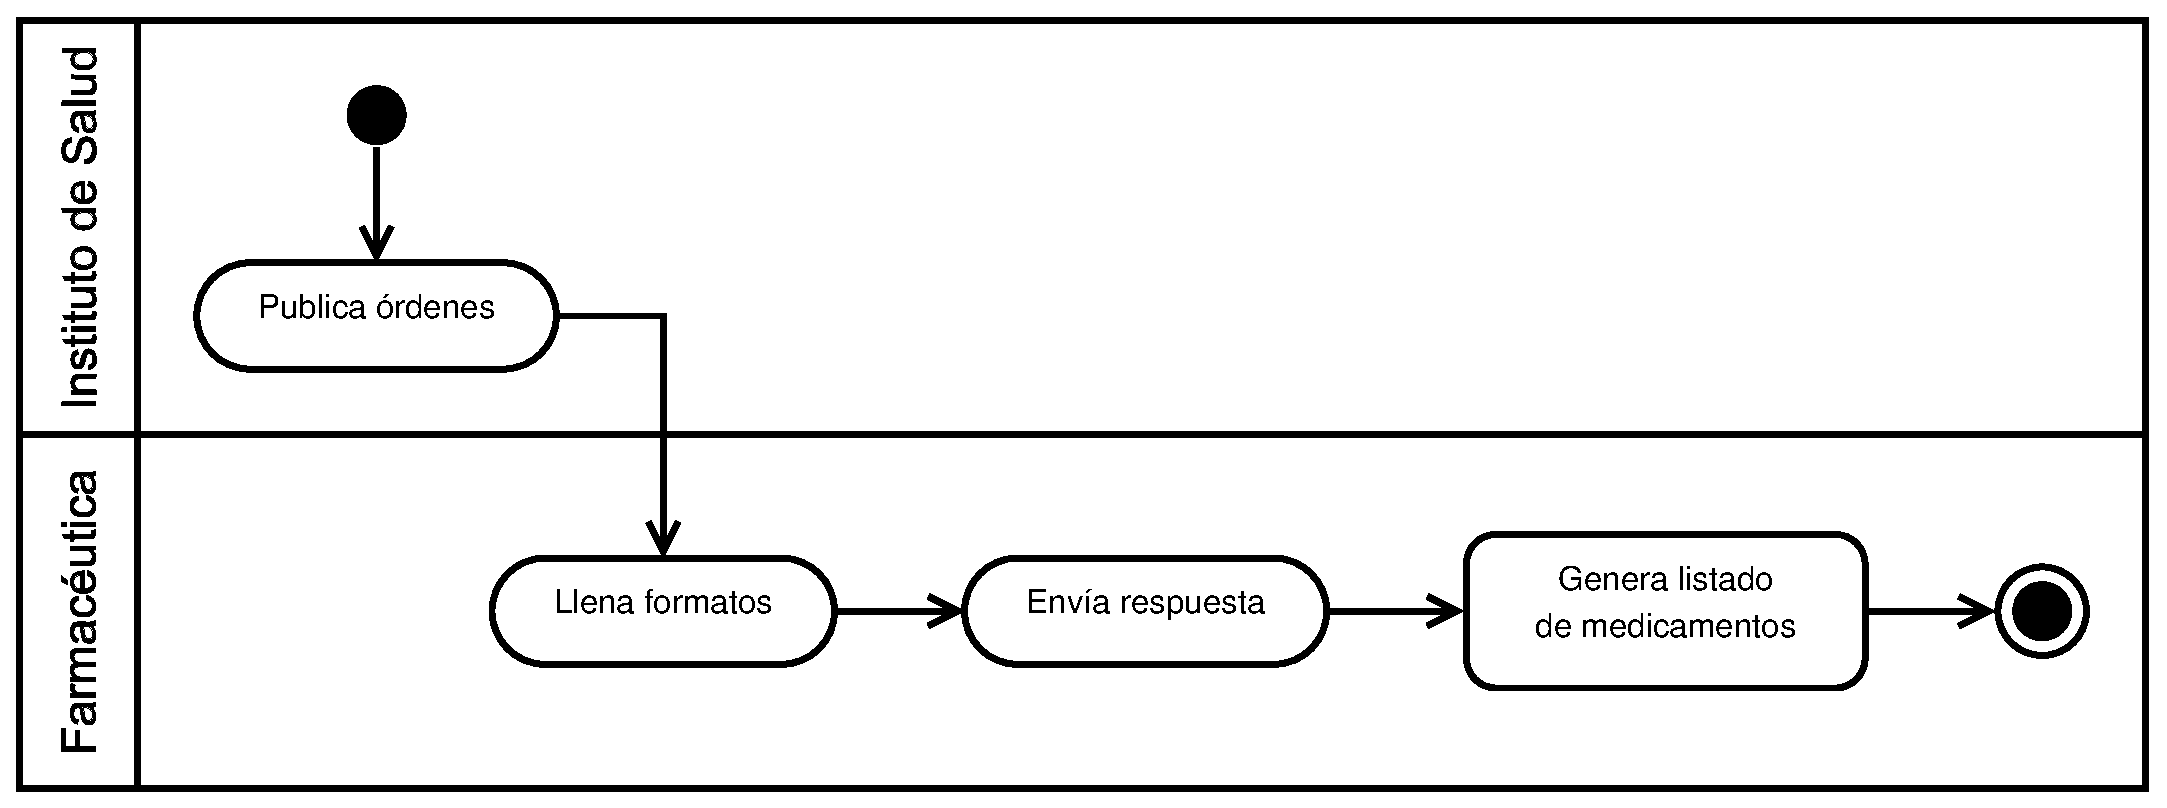
\includegraphics[width=\textwidth]{flow-proc-contestar} 
		\label{fig:flow-proc-contestar}
		\end{figure}
	\end{frame}

	\begin{frame}{Verificación de órdenes de reposición canceladas}
		\begin{figure}[H]
		\centering
		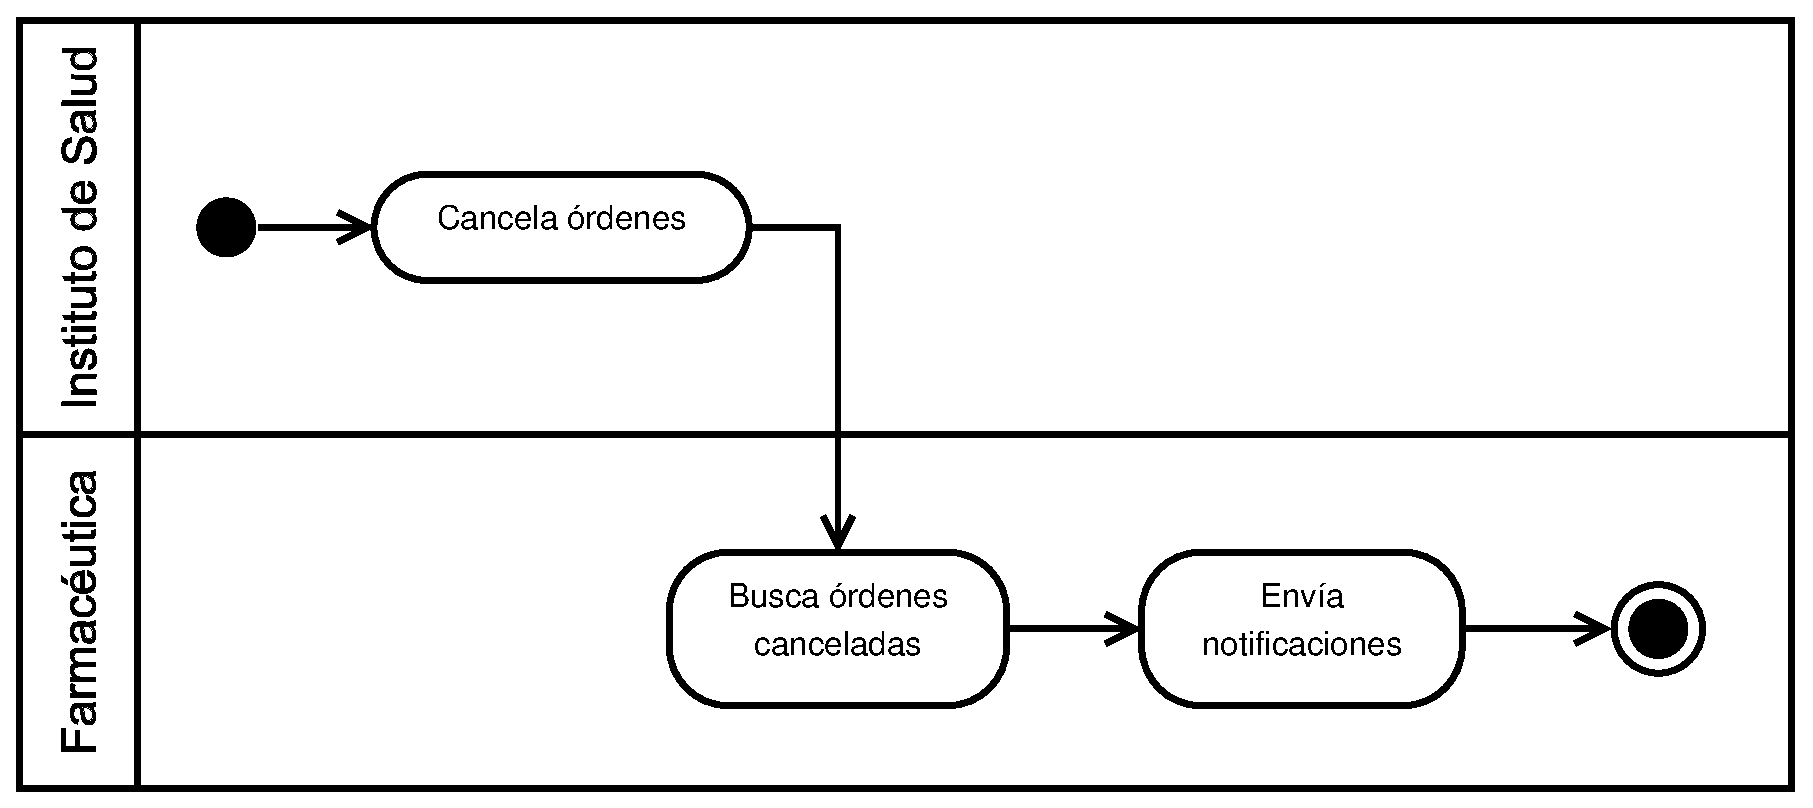
\includegraphics[width=\textwidth]{flow-proc-verificar} 
		\label{fig:flow-proc-verificar}
		\end{figure}
	\end{frame}

\subsection{Objetivos}
	\begin{frame}{Objetivo principal}
		Describir un sistema de cómputo que reduzca el tiempo de interacción entre los operadores de la farmacéutica y el \textit{Sistema de Abastecimiento}.
	\end{frame}

	\begin{frame}{Metas del objetivo principal}
		\begin{enumerate}
			\item Reducir el tiempo para contestar las órdenes de reposición.
			\item Evitar el envío de medicamentos no solicitados.
			\item Agilizar la generación de reportes.
		\end{enumerate}
	\end{frame}

	\begin{frame}{Objetivos secundarios}
		\begin{enumerate}
		\item Reducir el error humano en la manipulación de la información.
		\item Ahorrar recursos en la entrega de medicamentos no solicitados.
		\item Reducir el tiempo de respuesta a las órdenes de reposición.
		\item Dar consistencia en los datos de operación.
		\end{enumerate}
	\end{frame}

\subsection{Metodología de trabajo}
	\begin{frame}{Equipo de trabajo}
		\begin{block}{Metodología}
			Marco de trabajo \textit{Scrum}.
		\end{block}
		\begin{block}{Roles en el equipo de trabajo}
			\begin{enumerate}
				\item Arquitecto.
				\item Desarrollador.
			\end{enumerate}
		\end{block}
	\end{frame}

	\begin{frame}{Arquitecto}
		\begin{enumerate}
			\item Supervisar el diseño e implementación.
			\item Realizar investigación sobre herramientas.
			\item Cumplir con el rol de \textit{Scrum Master}.
			\item Formar parte del \textit{Scrum Team}.
		\end{enumerate}
	\end{frame}

	\begin{frame}{Desarrollador}
		\begin{enumerate}
			\item Levantar requerimientos.
			\item Realizar investigación sobre herramientas.
			\item Realizar diseño e implementación.
			\item Cumplir con el rol de \textit{Product Owner}.
			\item Formar parte del \textit{Scrum Team}.
		\end{enumerate}
	\end{frame}


\section{Análisis}
\subsection{Alcance}
	\begin{frame}{Alcance}
		\begin{block}{Dentro del alcance}
			\begin{itemize}
				\item Automatizar procesos en el \textit{Sistema de Abastecimiento}.
				\item Aplicación web para gestionar las órdenes atendidas.
				\item Generación de reportes.
			\end{itemize}
		\end{block}
		\begin{block}{Fuera del alcance}
			\begin{itemize}
				\item Integración con sistemas externos.
				\item Respaldo información.
				\item Seguridad con certificados SSL.
			\end{itemize}
		\end{block}
	\end{frame}

\subsection{Riesgos}
	\begin{frame}{Riesgos}
		\begin{enumerate}
			\item Falta de ambiente de pruebas.
			\item Cambios en la estructura de las páginas del \textit{Sistema de Abastecimiento}.
			\item La herramienta \textit{Sahi} en su versión libre no cuenta con soporte bajo demanda.
		\end{enumerate}
	\end{frame}

\subsection{Requerimientos funcionales}
	\begin{frame}{Requerimientos funcionales}
		\begin{block}{Automatización de procesos}
			\begin{enumerate}
				\item Respuesta a órdenes de reposición.
				\item Verificación de órdenes canceladas.
			\end{enumerate}
		\end{block}
		\begin{block}{Página web de administración}
			\begin{multicols}{2}
				\begin{enumerate}
					\item Acceso restringido.
					\item Búsqueda.
					\item Visualización.
					\item Actualización.
				\end{enumerate}
			\end{multicols}
		\end{block}
		\begin{block}{Generación de reportes}
			\begin{enumerate}
				\item Generación de reportes.
				\item Actualización de catálogos.
			\end{enumerate}
		\end{block}
	\end{frame}
	\begin{frame}{Automatización de la respuesta}
		\centering
		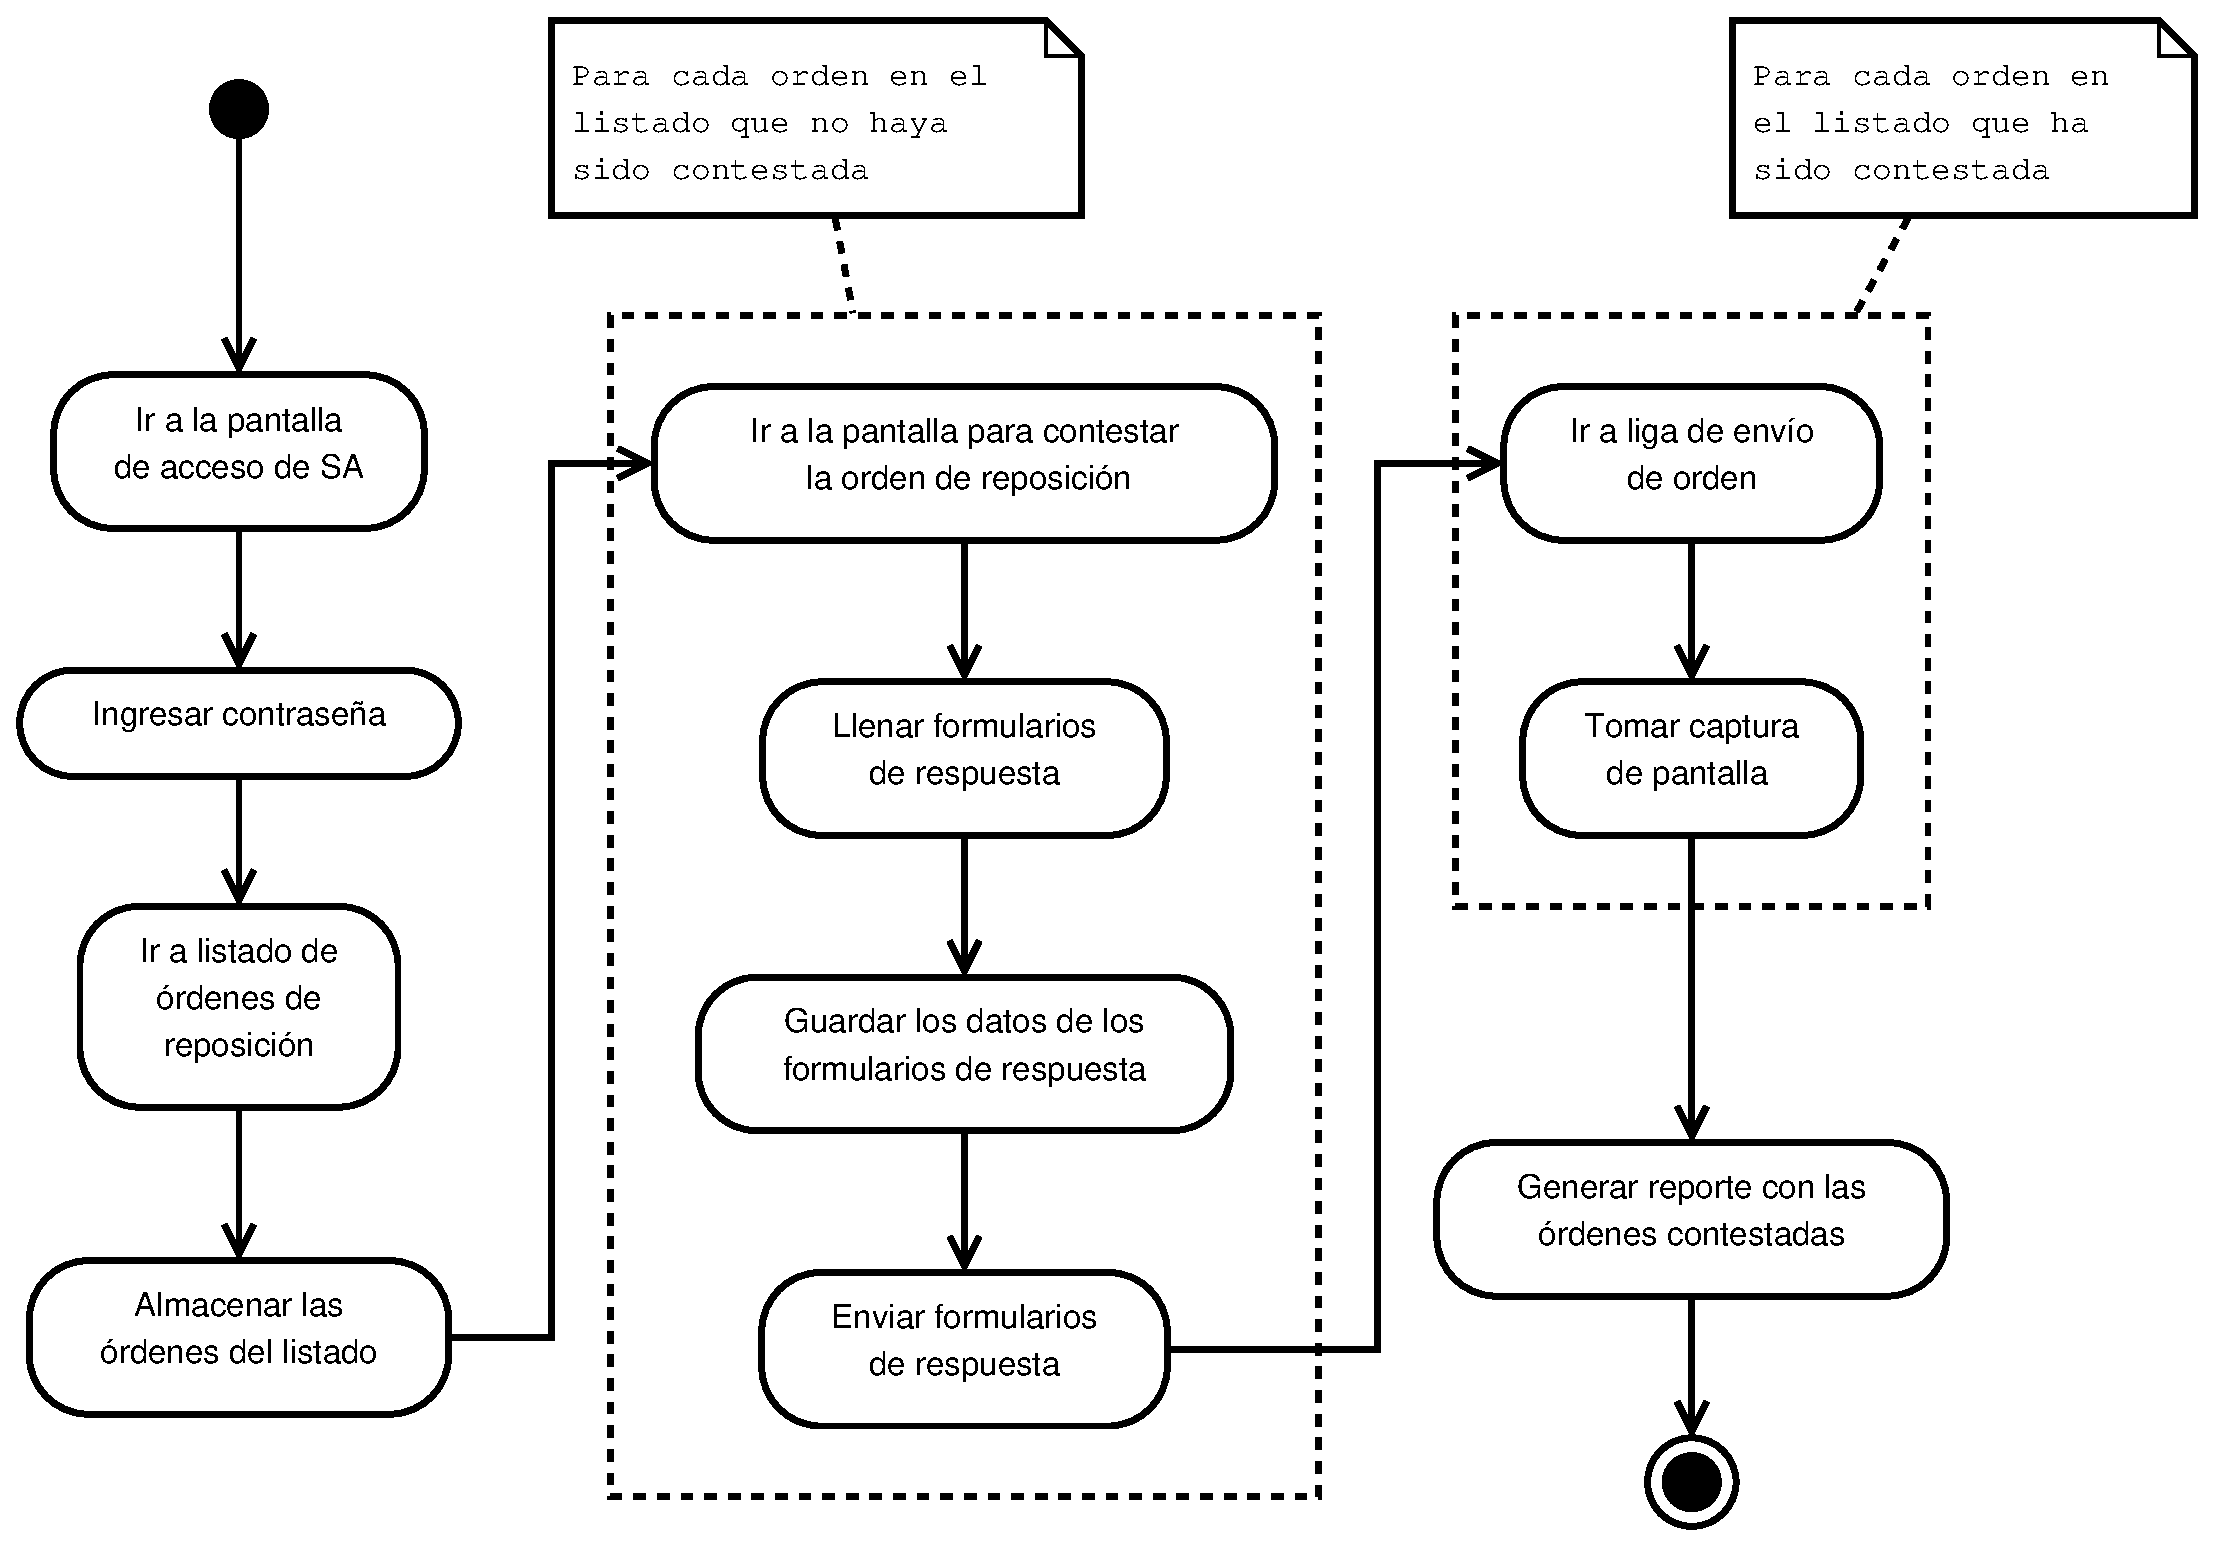
\includegraphics[scale=0.2]{dia-activity-contestar}
	\end{frame}
	\begin{frame}{Listado de órdenes de reposición}
		\begin{figure}[H]
		\centering
		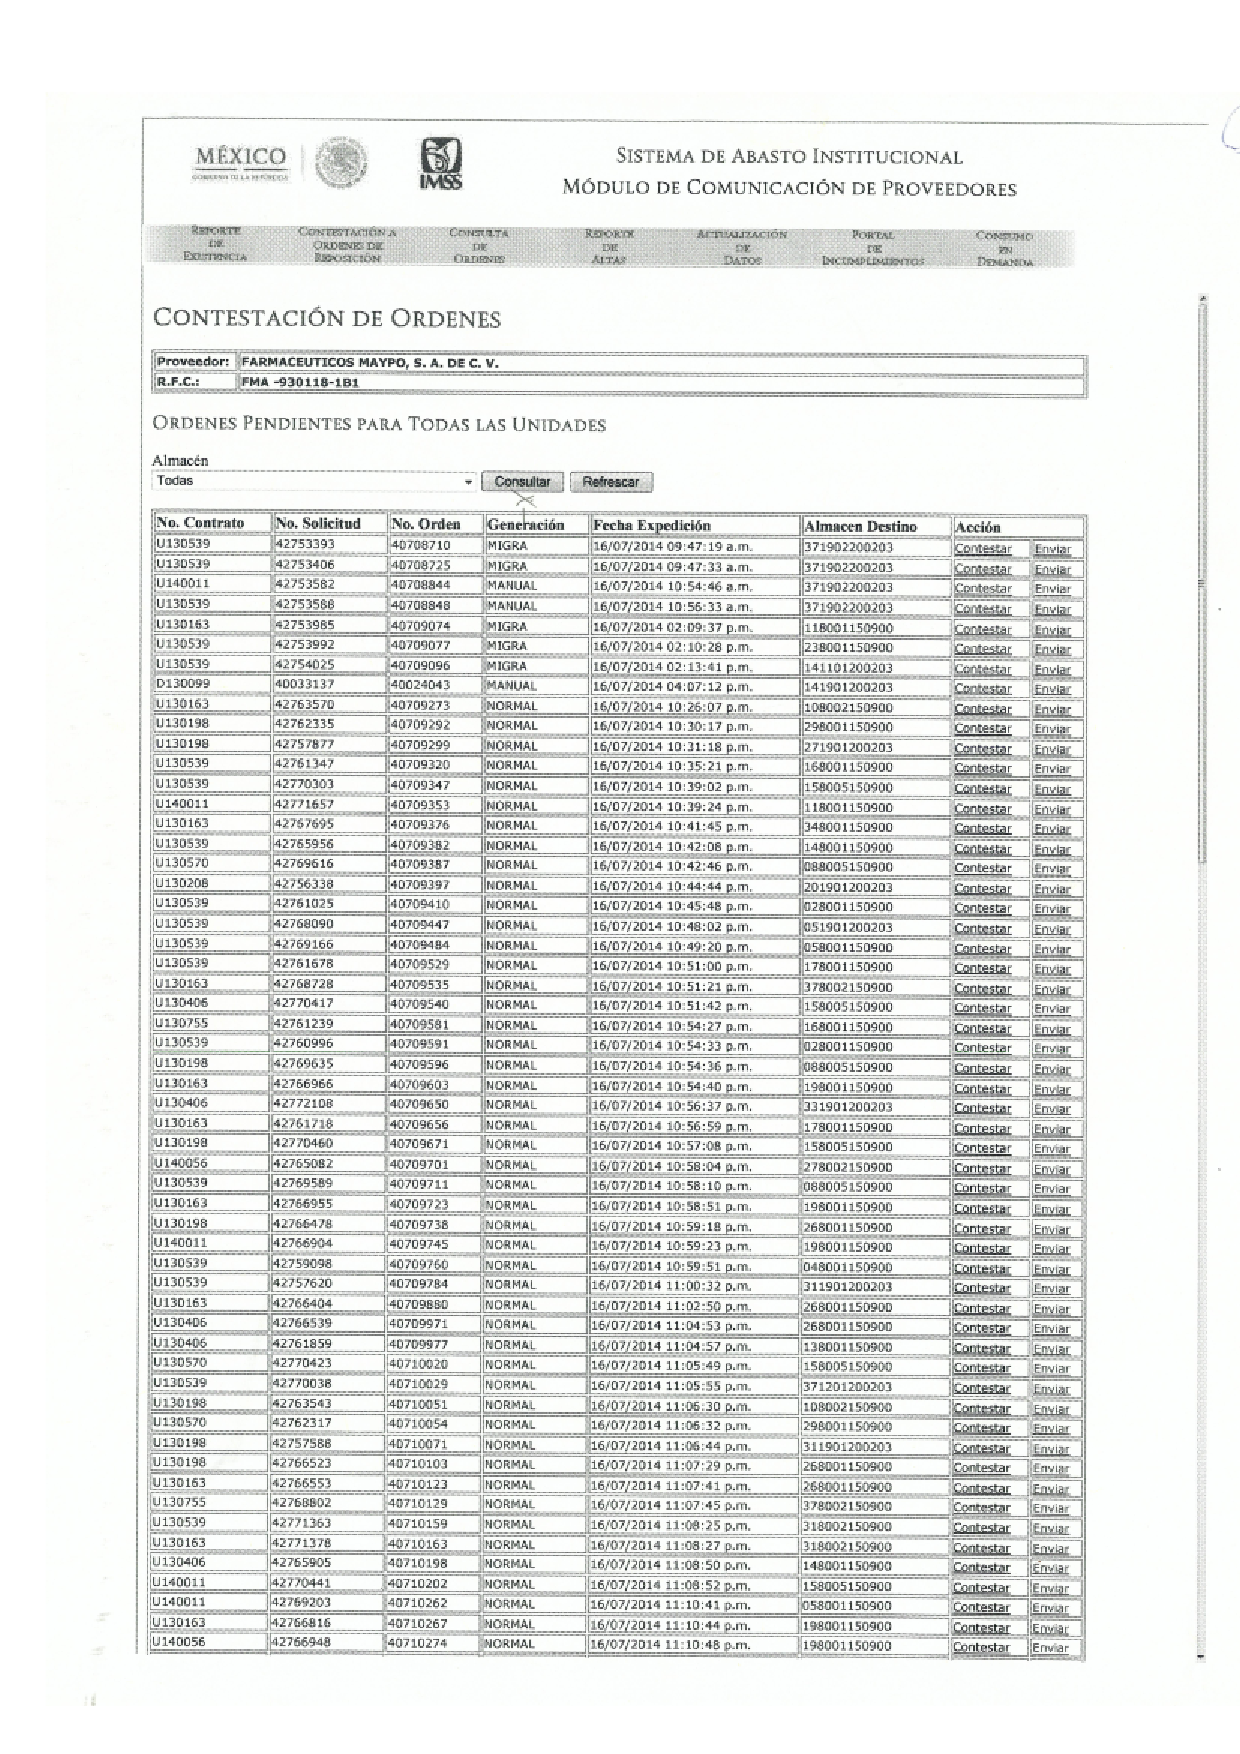
\includegraphics[width=\textwidth]{sai1}
		\label{fig:sai1}
		\end{figure}
	\end{frame}
	\begin{frame}{Respuesta a una orden de reposición}
		\begin{figure}[H]
		\centering
		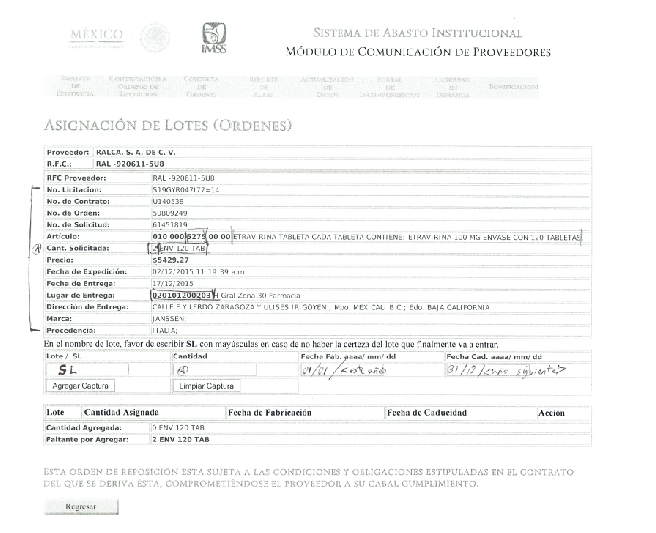
\includegraphics[scale=0.8]{sai2}
		\label{fig:sai2}
		\end{figure}
	\end{frame}
	\begin{frame}{Envío de una orden de reposición}
		\begin{figure}[H]
		\centering
		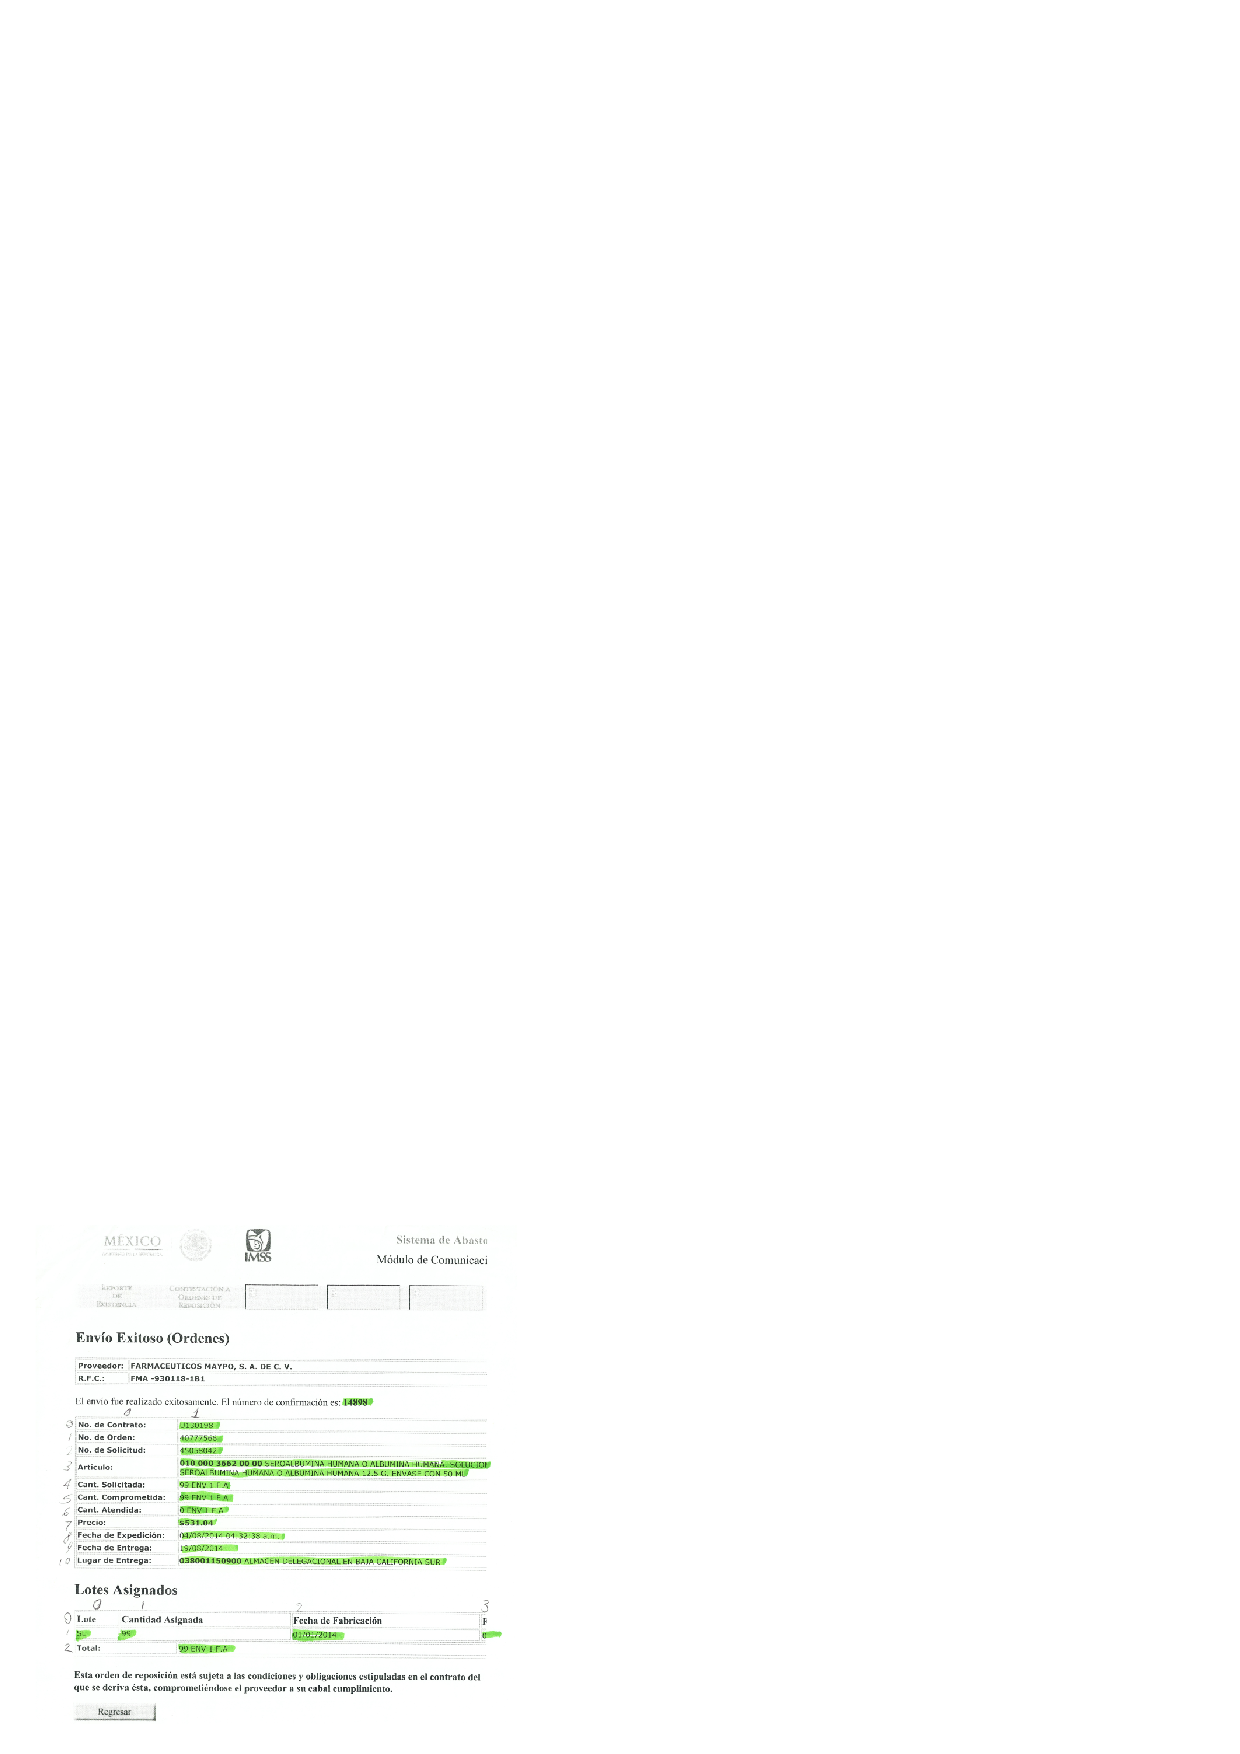
\includegraphics[scale=0.9]{sai4}
		\label{fig:sai4}
		\end{figure}
	\end{frame}
	\begin{frame}{Formato de salida}
		\begin{figure}[H]
		\centering
		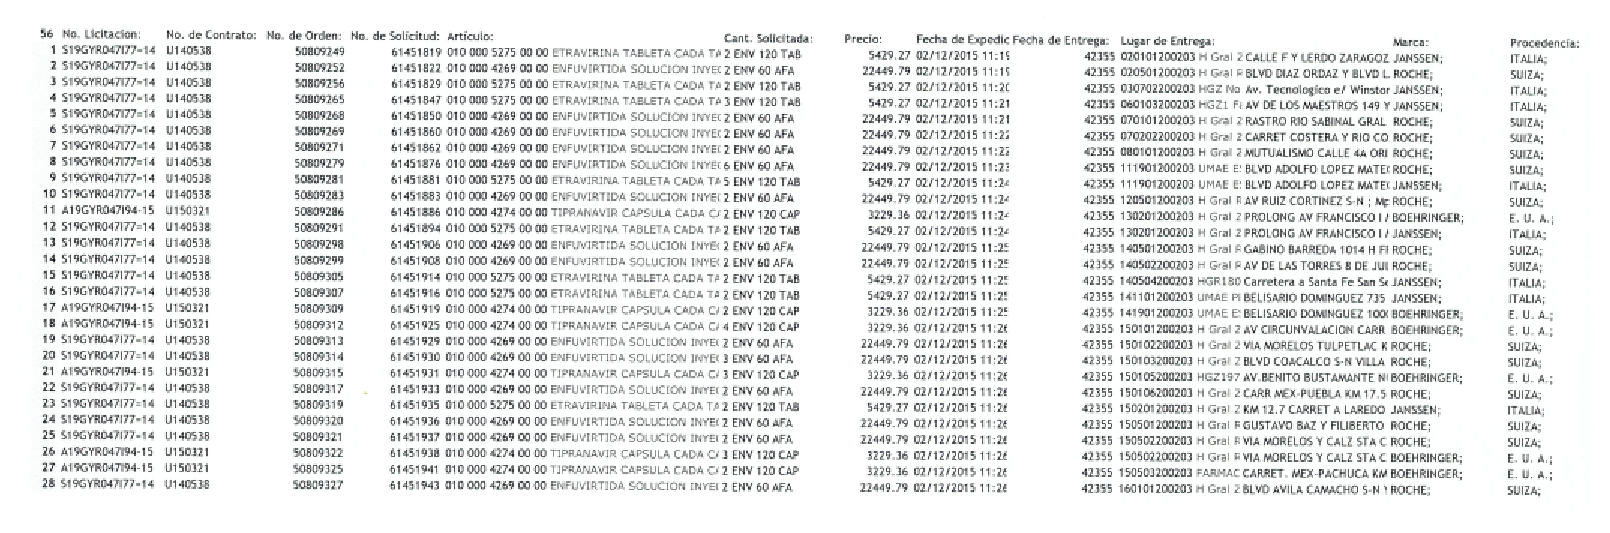
\includegraphics[width=\textwidth]{sai5}
		\label{fig:sai5}
		\end{figure}
	\end{frame}
	\begin{frame}{Diagrama de estados de las órdenes}
		\centering
		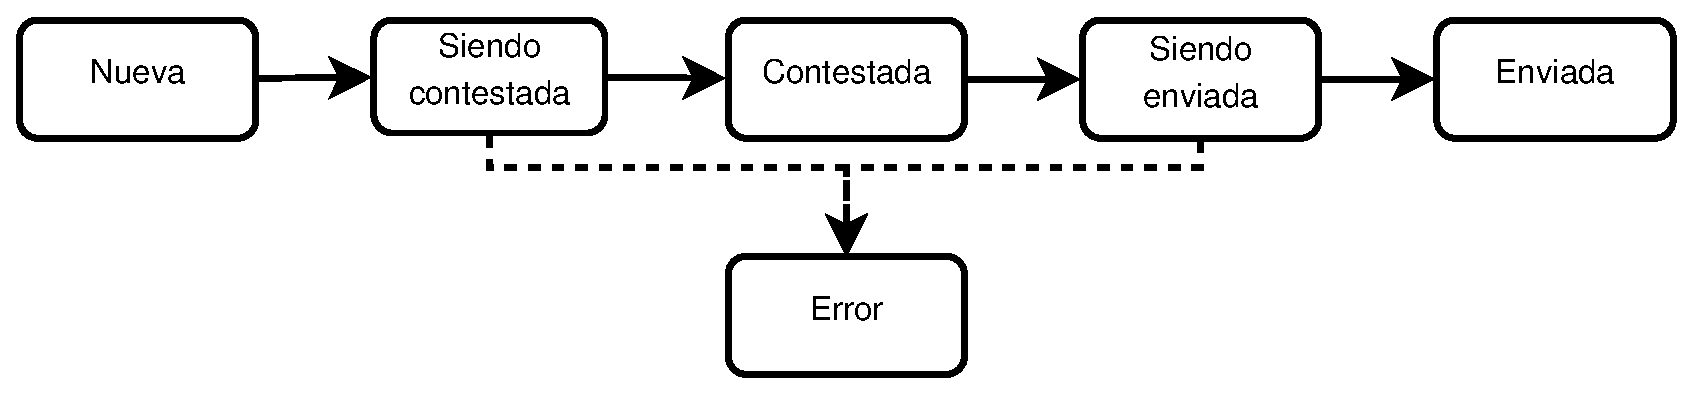
\includegraphics[width=\textwidth]{dia-estados-orden} 
	\end{frame}
	\begin{frame}{Automatización de la verificación}
		\centering
		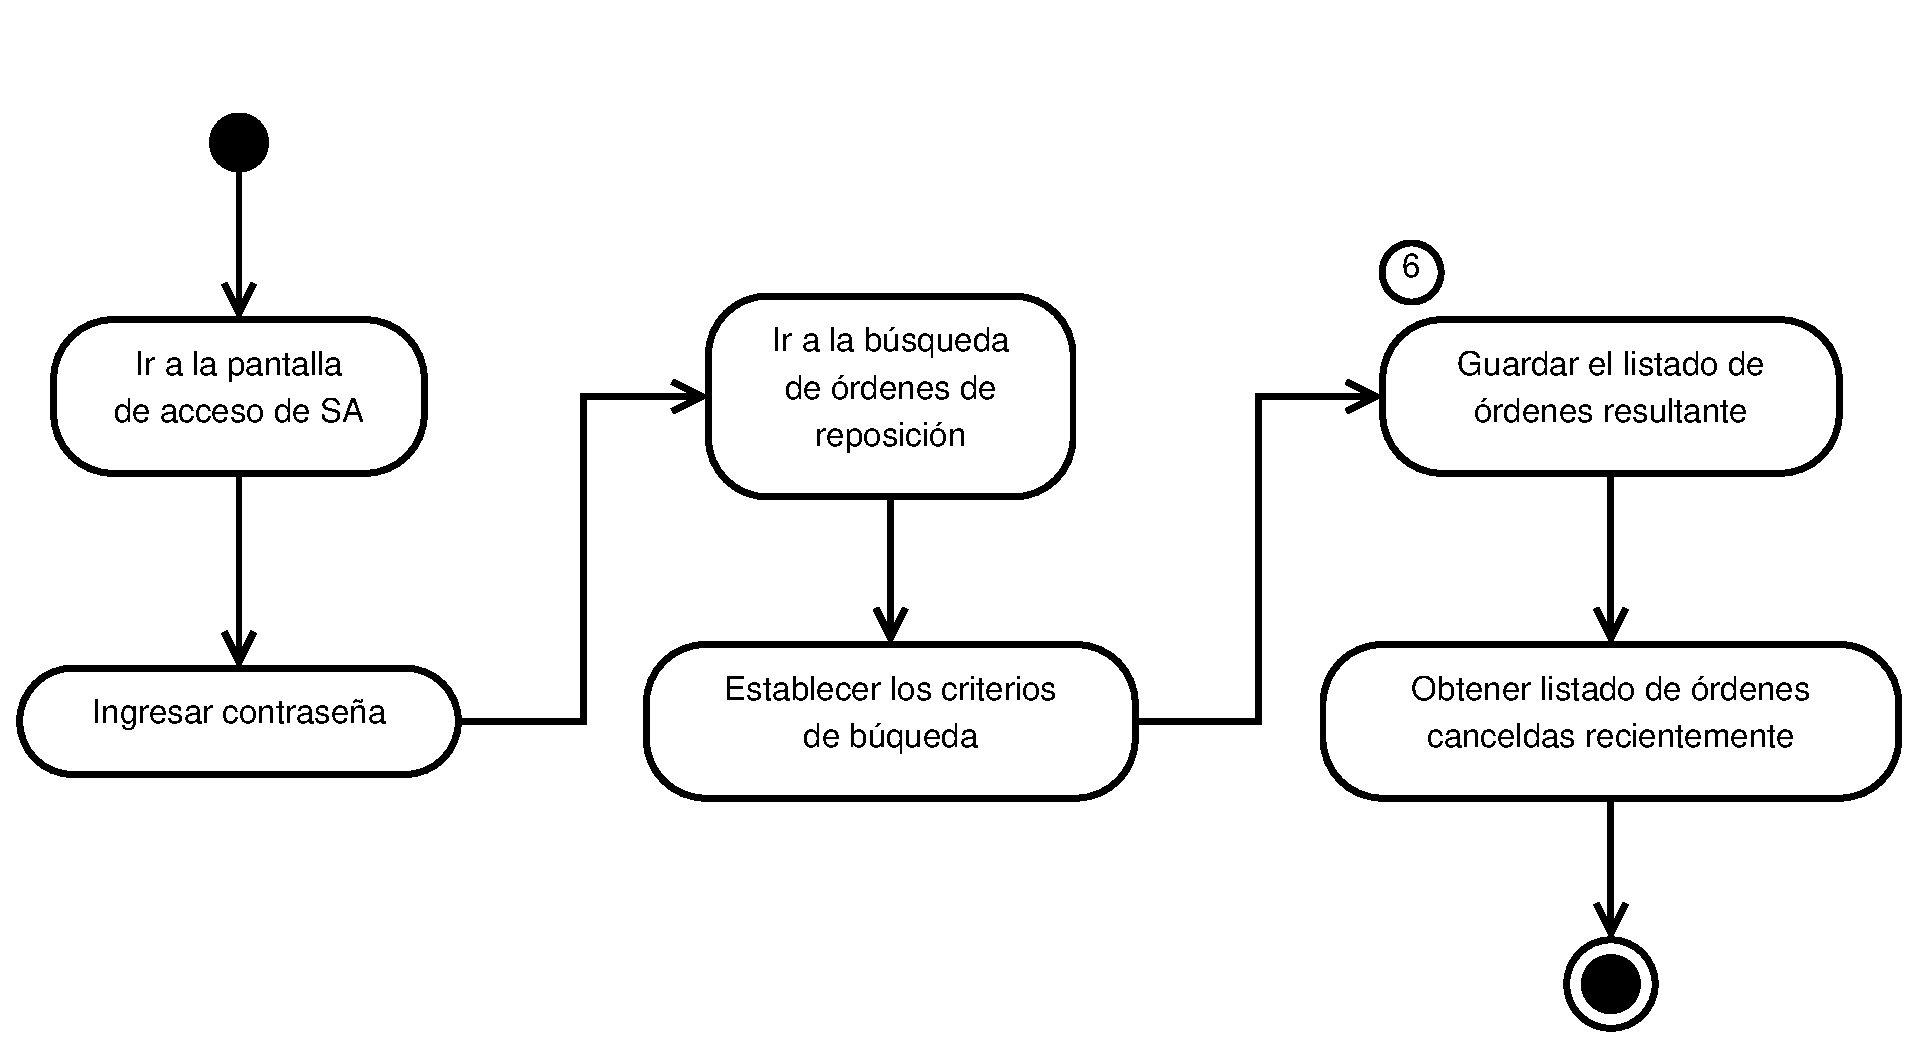
\includegraphics[width=\textwidth]{dia-activity-verificar}
	\end{frame}
	\begin{frame}{Navegación en la interfaz web}
		\centering
		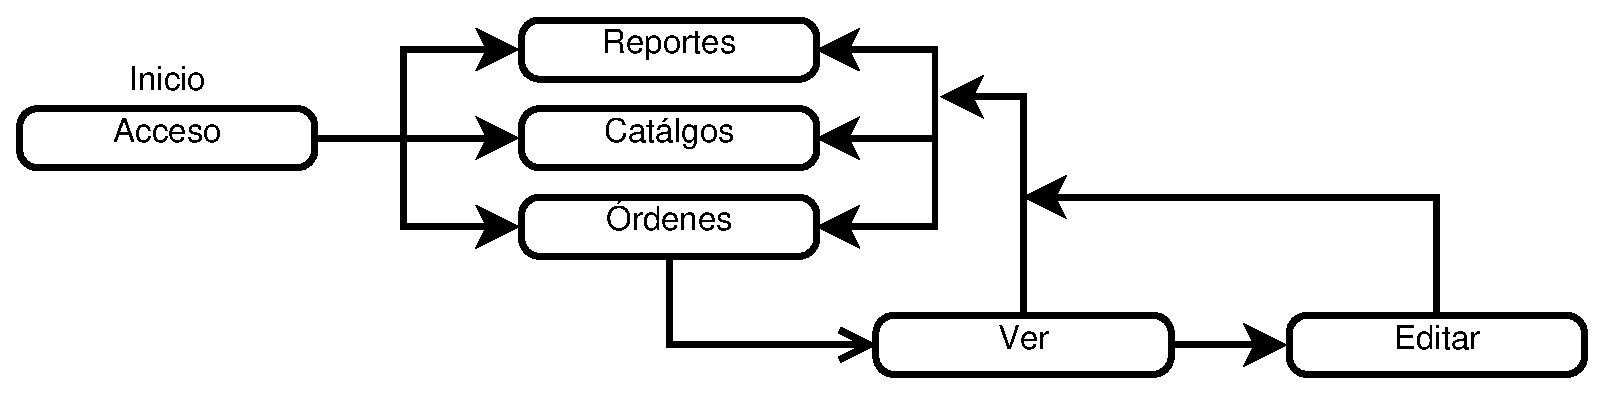
\includegraphics[scale=0.4]{dia-nav-flow}
	\end{frame}
	\begin{frame}{Acceso a la interfaz web}
		\centering
		
\includegraphics[scale=0.5]{maq-login} 
	\end{frame}
	\begin{frame}{Búsqueda de órdenes}
		\centering
		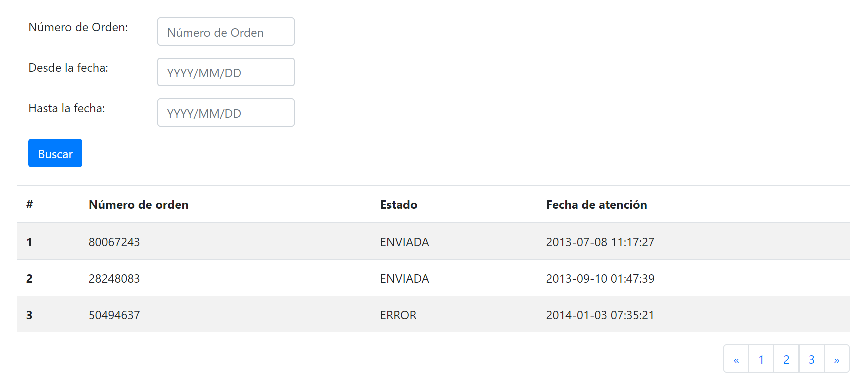
\includegraphics[width=\textwidth]{maq-search} 
	\end{frame}
	\begin{frame}{Visualización/Edición}
		\centering
		
\includegraphics[scale=1]{maq-crud} 
	\end{frame}
	\begin{frame}{Generación de reportes}
		\centering
		
\includegraphics[scale=1.2]{maq-report} 
	\end{frame}
	\begin{frame}{Actualización de catálogos}
		\centering
		
\includegraphics[scale=1.3]{maq-upload}
	\end{frame}

\subsection{Requerimientos no funcionales}
	\begin{frame}{Requerimientos no funcionales}
		\begin{enumerate}
			\item Ejecución en sistema operativo Windows\textsuperscript{\textcopyright} o Unix.
			\item Base de datos relacional SQL.
			\item Uso de la herramienta \textit{Sahi}.
			\item Cifrado de contraseñar.
		\end{enumerate}
	\end{frame}

\subsection{Casos de uso}
	\begin{frame}{Casos de uso}
		\centering
		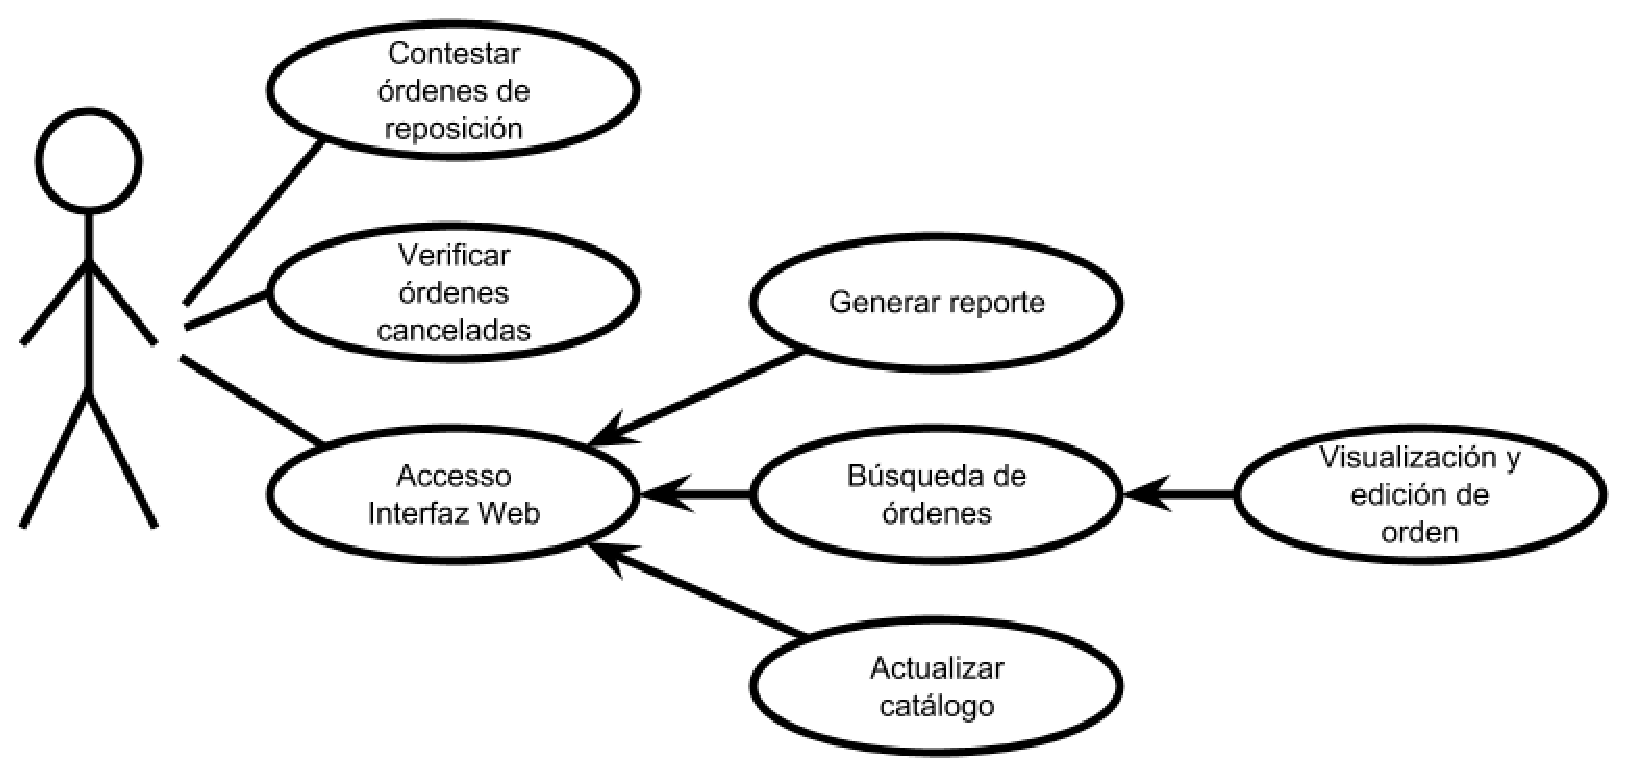
\includegraphics[scale=0.35]{dia-casos-uso} 
	\end{frame}



%\section{Diseño e implementación}
\subsection{Productos ejecutables}
	\begin{frame}{Productos ejecutables}
		\begin{enumerate}
		 	\item Rutinas automatizadas: se ejecutan a partir del entorno gráfico del sistema operativo.
		 	\item Portal de usuario: se ofrece como una página web, la cual depende del servidor web de la farmacéutica y del explorador web del usuario.
		\end{enumerate}
	\end{frame}
	\begin{frame}{Automatización de rutinas}
		\begin{figure}[h]
		\centering
		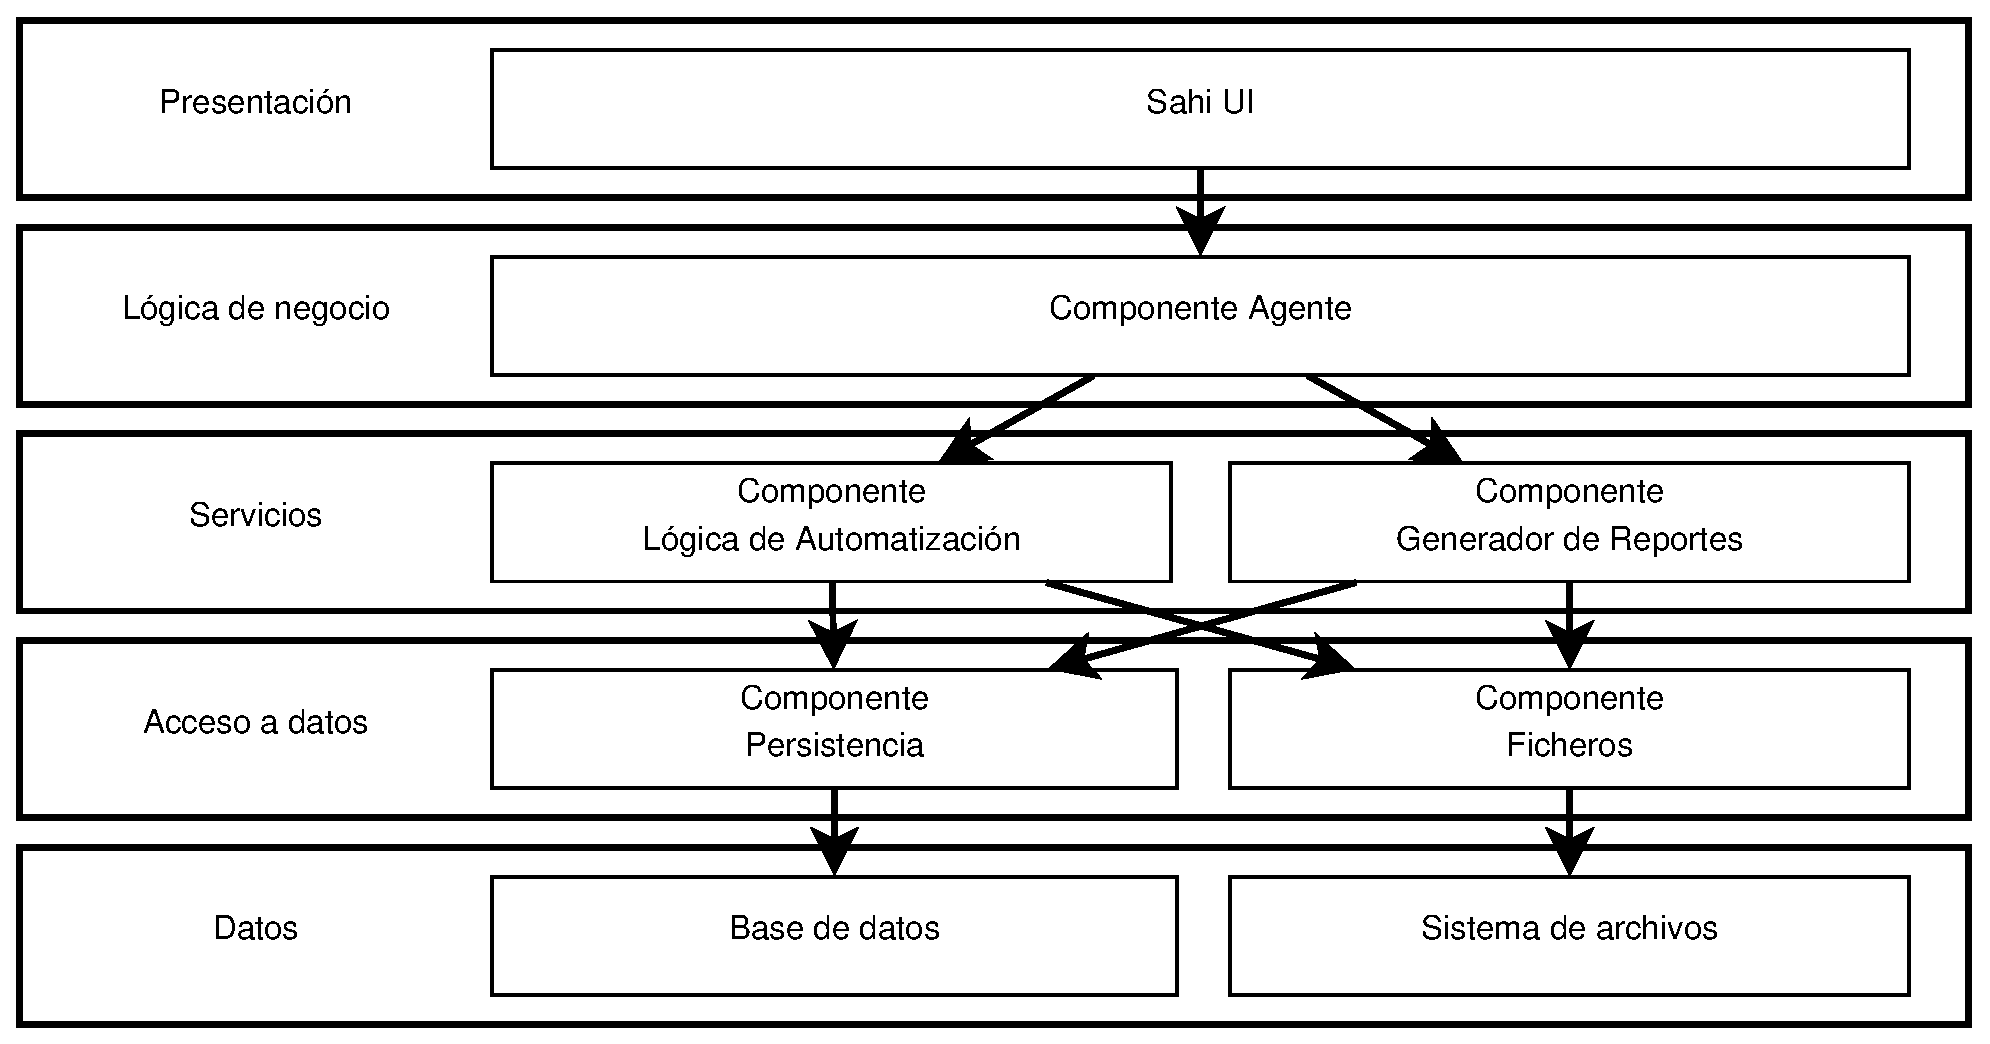
\includegraphics[width=\textwidth]{dia-layers-auto}
		\label{fig:dia-layers-auto}
		\end{figure}
	\end{frame}
	\begin{frame}{Aplicación web}
		\begin{figure}[h]
		\centering
		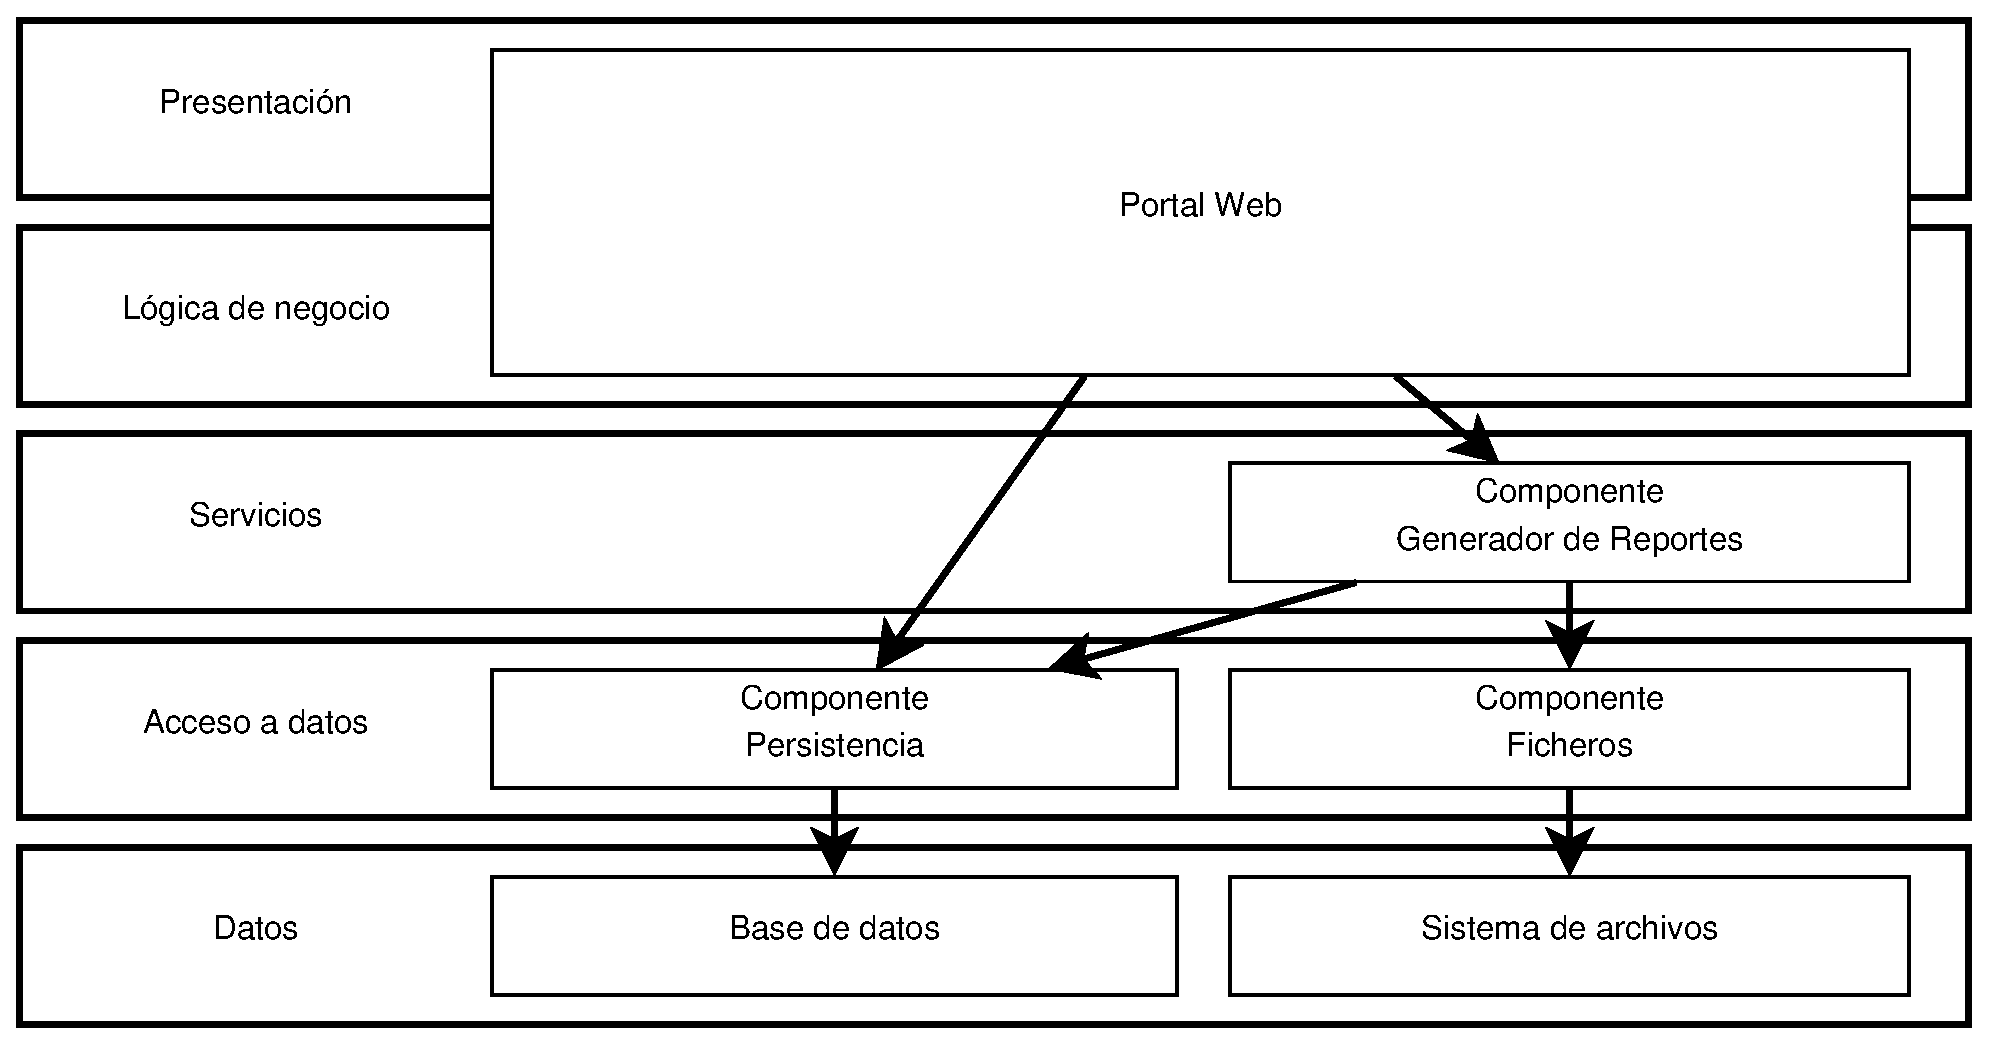
\includegraphics[width=\textwidth]{dia-layers-web}
		\label{fig:dia-layers-web}
		\end{figure}
	\end{frame}

\subsection{Componentes de AutoSA}
	\begin{frame}{Componentes de AutoSA}
		\centering
		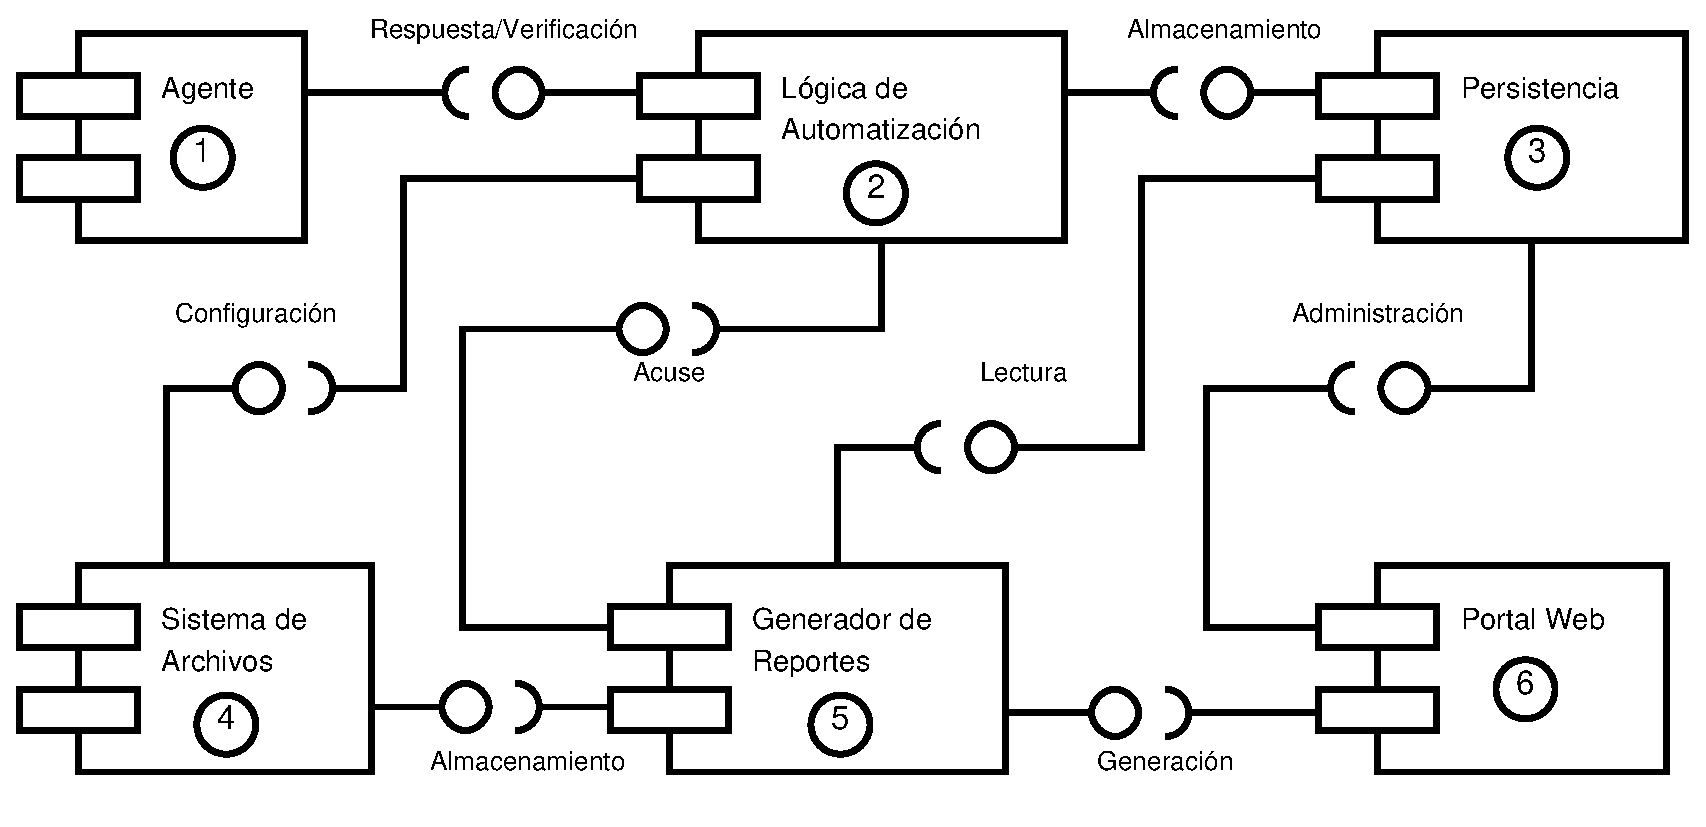
\includegraphics[width=\textwidth]{dia-components}
	\end{frame}

\subsection{Diagrama de paquetes}
	\begin{frame}{Diagrama de paquetes}
		\centering
		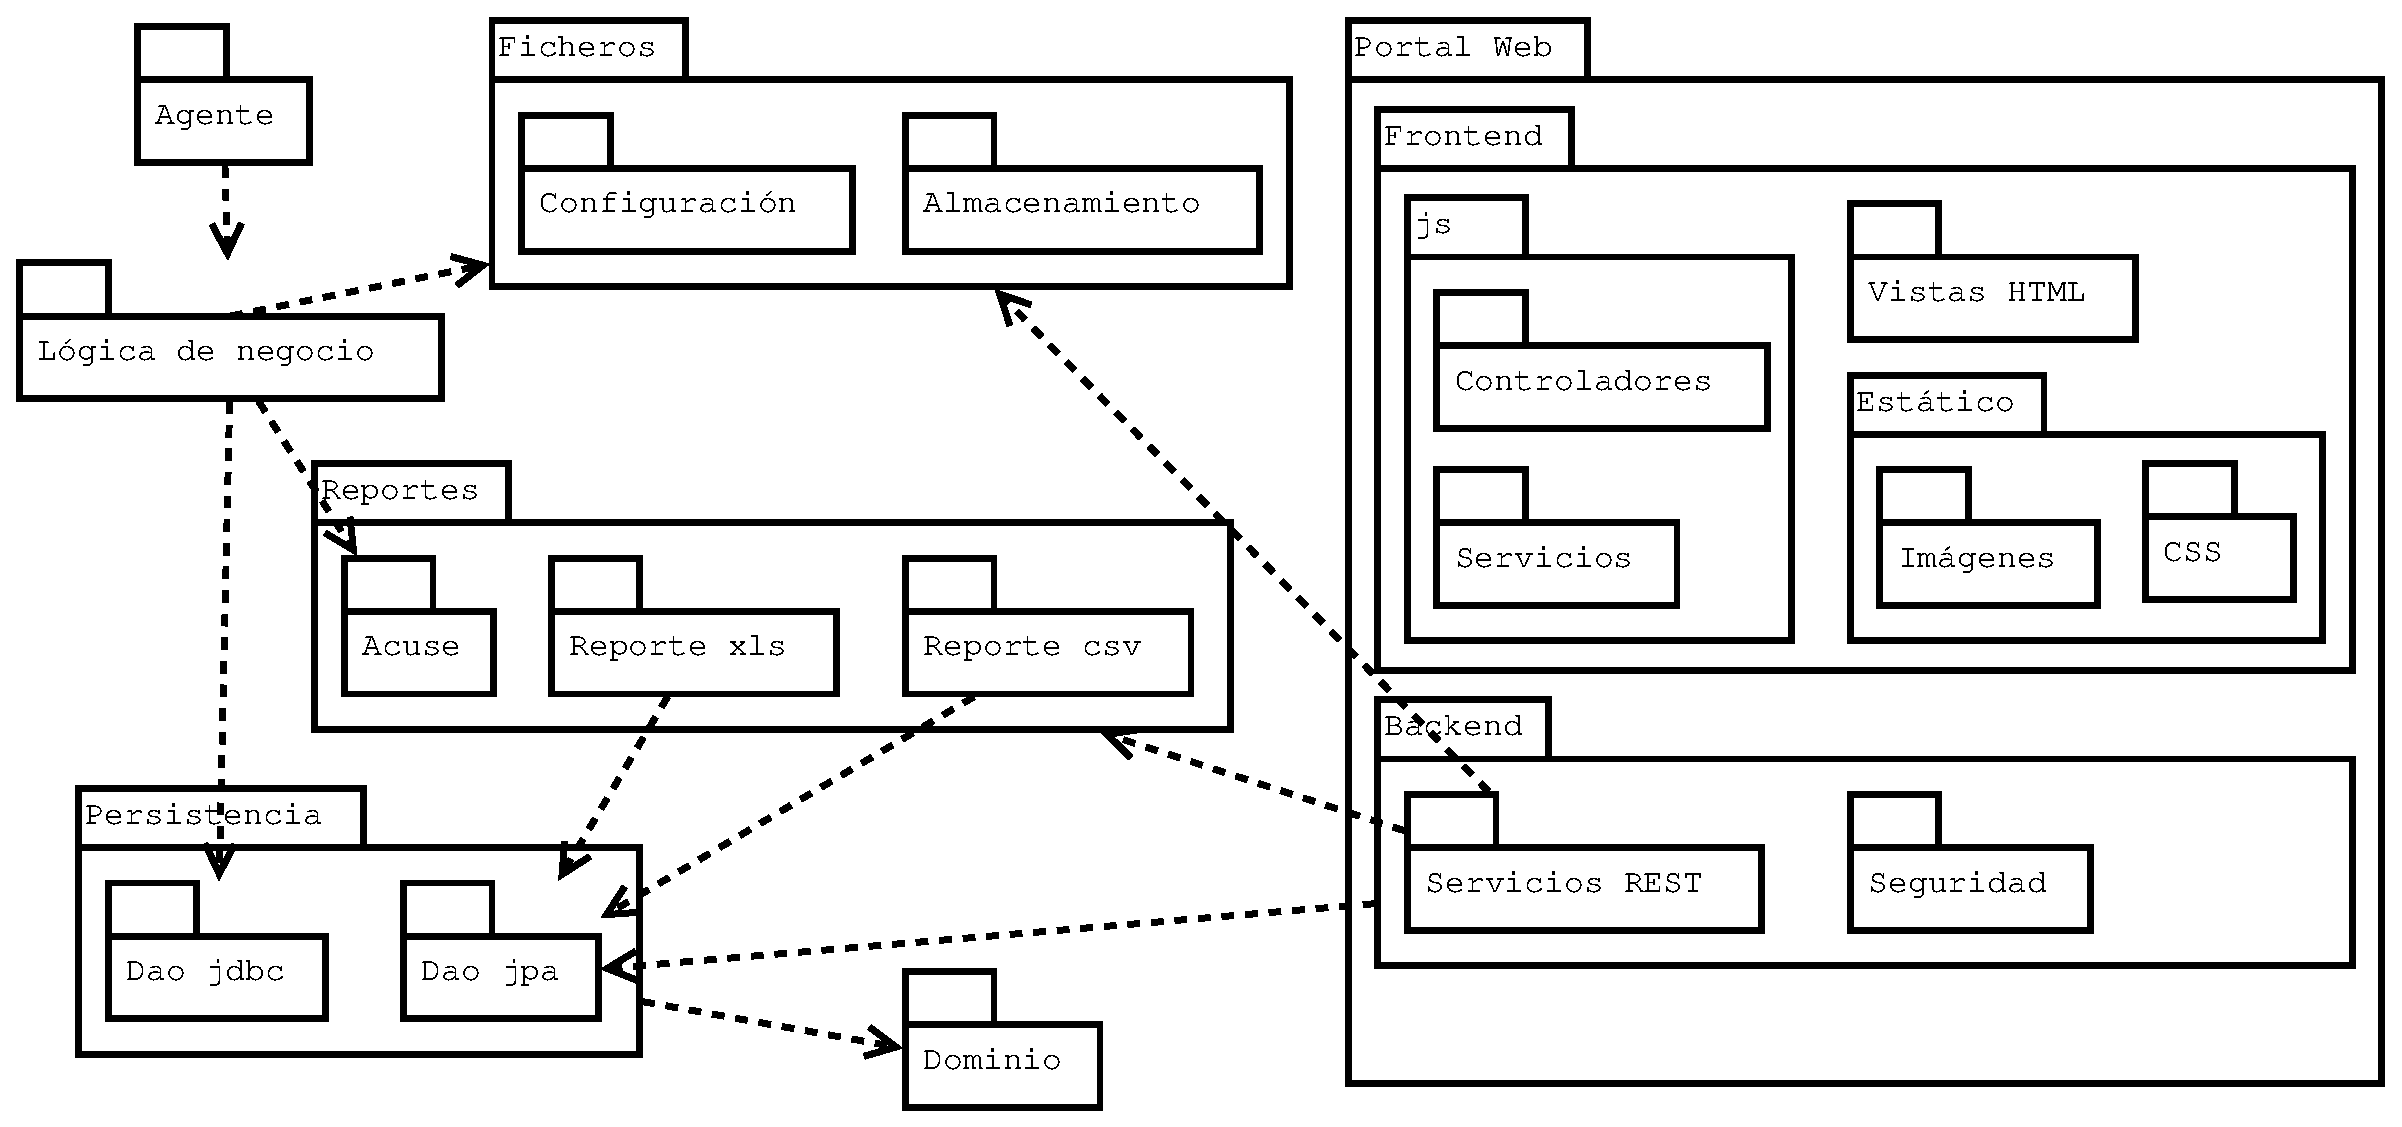
\includegraphics[width=\textwidth]{dia-package-large}
	\end{frame}


%\include{presentation-files/sections/implementation}

%\section{Resultados}
	\begin{frame}{Resultados}
		\begin{enumerate}
			\item Reducción del tiempo de respuesta.
			\item Reducción de horas extras de los empleados de la farmacéutica.
			\item Reducción del error humano.
			\item Ahorro de recursos en la entrega de medicamentos no solicitados.
		\end{enumerate}
	\end{frame}

	\begin{frame}{Comparación de tiempo de interacción con el Sistema de Abastecimiento}
		\begin{columns}[t]
			\column{0.5\textwidth}
			\begin{block}{Previo a AutoSA}
				\begin{enumerate}
					\item 3 personas al día.
					\item 24 horas hombre.
					\item Verificación de canceladas cada 3 días.
				\end{enumerate}
			\end{block}

			\column{0.5\textwidth}
			\begin{block}{Con AutoSA}
				\begin{enumerate}
					\item 1 persona al día.
					\item 1.5 horas hombre.
					\item Verificación de canceladas cada día.
				\end{enumerate}
			\end{block}
		\end{columns}
	\end{frame}

	\begin{frame}{Rendimiento de AutoSA}
		\begin{itemize}
			\item Liberado en diciembre de 2014. 
			\item No se han reportado errores hasta octubre de 2019.
			\item Vendido a otra farmacéutica en diciembre de 2015.
		\end{itemize}
	\end{frame}

	\begin{frame}{Sinodales}
		\begin{itemize}
			\item M. en I. Karla Ramírez Pulido.
			\item M. en C. María Guadalupe Elena Ibargüengoitia González.
			\item Dra. Hanna Jadwiga Oktaba.
			\item M. en I. Beatriz Peralta Cortés.
			\item L. en C.C. Oscar Ruiz Salinas.
		\end{itemize}
	\end{frame}

	\begin{frame}
		\centering
		\huge{¡Muchas Gracias!}
	\end{frame}


\end{document}


